Steigende Anforderungen an die Produktqualität und immer kürzer werdende Entwicklungszei-ten erfordern stetige Verbesserungen im Produktentstehungsprozess. Eine Schlüsselrolle kommt dabei der Systembeschreibung und der Systemsimulation zu. Systemsimulationen lassen sich erheblich schneller und reproduzierbarer umsetzen als der Aufbau von Musterteilen. Aus diesem Grund steigt in der Produktentwicklung der Anteil von Simulationsaufgaben an. Ingenieure be-nötigen damit ein interdisziplinäres Systemverständnis, mit dem komplexe Systeme erfasst, be-schrieben und simuliert werden können.\newline
Unter einem System wird die Abstraktion eines Prozesses oder Gebildes verstanden, das mehrere Signale zueinander in Verbindung setzt. Systeme sind dabei oft interdisziplinär, sie erstrecken sich über mehrere Fachrichtungen. Einige dieser Systeme lassen sich direkt mit algebraischen Gleichungen \newline beschreiben. Ein Beispiel für ein solches System ist ein Spannungsteiler, bei dem sich Ausgangsspannung direkt aus der Eingangsspannung und dem Widerstandsverhältnis ergibt. Oftmals finden bei praktischen Anwendungen aber Einschwingvorgänge statt. Sie ergeben sich aus Energiespeichern, deren Zustand sich durch eine Anregung zeitabhängig ändert. Ein Beispiel für ein System mit Energiespeicher ist ein Kondensator, der über einen Widerstand aufgeladen wird. Die Ausgangsspannung des Kondensators ist zeitabhängig. Systeme mit Energiespeichern werden als dynamische Systeme bezeichnet. Andere bekannte Beispiele für dynamische Syste-me sind Pendelbewegungen, das Verhalten elektrischer Schaltungen mit Kondensatoren und Spulen sowie thermische und chemische Prozesse. Es wird sich zeigen, dass die Systembe-schreibung bei dynamischen Systemen aus einer oder mehreren Differentialgleichungen besteht.\newline
Die Systemtheorie liefert eine Theorie zur einheitlichen Beschreibung von dynamischen Syste-men, die sehr unterschiedlicher Natur sein können. Insbesondere für regelungstechnische An-wendungen ist die Systemtheorie damit eine wesentliche Voraussetzung, da sie Systeme in einer einheitlichen Weise beschreibt. Weitere Anwendungen in der Ingenieurwissenschaft sind die Automatisierungstechnik, Nachrichtentechnik, Messtechnik, Verfahrenstechnik, Informatik so-wie die klassische Elektrotechnik. In aller Regel werden abstrakte Systembeschreibungen mit Verzicht auf das Detail eingesetzt. Teilweise werden die Systembeschreibungen durch detaillierte Modelle kritischer Teilsysteme ergänzt. Durch die abstrakte Beschreibungsform bleibt der Über-blick über das System erhalten. 

\clearpage

\subsection{Strukturierung des Buchs }

In der Systemtheorie werden Systeme und ihre Wirkung auf Signale beschrieben. Deshalb wer-den in Kapitel 2 zunächst wesentliche Beschreibungsformen für Signale im Zeitbereich wieder-holt. Es werden sogenannte Sprung- und Impulsfunktionen definiert, die bevorzugte Testsignale dynamischer Systeme sind. Das Einschwingverhalten wird in vielen Fällen durch abklingende harmonische Schwingungen beschrieben, die als komplexe Exponentialfunktionen beschrieben werden.\newline
Einführende Beispiele in Kapitel 3 zeigen, dass viele zeitkontinuierliche Systeme über Differentialgleichungen beschrieben werden. Eine besondere Stellung nehmen dabei lineare, zeitinvarian-te Systeme ein. Ihre Systemreaktion lässt sich im Zeitbereich auf verschiedene Arten bestimmen. Neben der direkten Lösung der Differentialgleichung wird die Berechnung der Systemantwort über das Superpositionsprinzip und Faltungsintegral bestimmt. Die Zweiteilung von Signalen und Systemen zieht sich weiter durch das Buch. \newline
Zur Lösung von Differentialgleichungen wird in Kapitel 4 die Laplace-Transformation einge-führt. Nach der Diskussion der Laplace-Transformation für Signale werden in Kapitel 5 Differentialgleichungen mithilfe der Laplace-Transformation gelöst, und es wird der Begriff der Über-tragungsfunktion zeitkontinuierlicher Systeme eingeführt. An der Übertragungsfunktion können wichtige Systemeigenschaften direkt abgelesen werden, ohne die Systemantwort ausrechnen zu müssen. Die Interpretation der Übertragungsfunktion wird beschrieben und an Beispielen ange-wendet. In der Elektrotechnik kommt der Beschreibung von RLC-Schaltkreisen eine besondere Bedeutung kommt zu. Sie wird als eine Anwendung der Laplace-Transformation ausführlich diskutiert.\newline
Die Fourier-Reihe beschreibt periodische Signale näherungsweise mit einer Grundschwingung und ihren Oberschwingungen. Mit ihr wird in Kapitel 6 der Begriff des Spektrums eingeführt. Es wird darüber hinaus gezeigt, wie mithilfe der Fourier-Transformation nichtperiodische Signale im Frequenzbereich beschrieben werden können. Dabei werden die Parallelen zwischen Fourier-Reihe und Fourier-Transformation sowie Laplace- und Fourier-Transformation herausgearbeitet. Anschließend wird in Kapitel 7 die Fourier-Transformation zur Interpretation von Systemen im Frequenzbereich herangezogen. \newline
Durch den Einsatz von Filtern werden in der Elektrotechnik erwünschte Spektralanteile von unerwünschten Spektralanteilen getrennt. Die Grundlagen zum Entwurf und zur Realisierung von Filterschaltungen werden in Kapitel 8 erarbeitet. Dabei wird allgemein auf die Zielsetzung der Filterentwicklung eingegangen, und es werden spezielle Filterentwurfsverfahren vorgestellt. Au-ßerdem werden aktive und passive Schaltungen für die Realisierung unterschiedlicher Filterent-würfe angegeben.\newline
Die lineare Systemtheorie ermöglicht die Systembeschreibung durch Strukturschaubilder, die aus vernetzten Übertragungsgliedern bestehen. Die dabei verwendeten Übertragungsglieder werden insbesondere in der Regelungstechnik eingesetzt. Wesentliche Übertragungsglieder werden in Kapitel 9 vorgestellt und ihr Zeit- und Frequenzverhalten zusammengefasst. \newline
In der modernen Regelungstechnik werden Systeme im sogenannten Zustandsraum beschrieben. Dabei ist jeder Koordinate des Zustandsraums eine Zustandsgröße zugeordnet, die den Zustand eines Energiespeichers des Systems beschreibt. Die Eingangs- und Ausgangssignale sowie die Zustandsgrößen sind Funktionen der Zeit. Diese Darstellung kommt damit der praktischen Vor-stellung näher als ihre Darstellung im Laplace- oder Fourier-Bereich. Die Darstellung von Syste-men im Zustandsraum wird in Kapitel 10 eingeführt.\newline
Kapitel 11 beschreibt einen Leitfaden zur Modellbildung von Systemen. Es wird aufgezeigt, wie mit dem gewonnenen Wissen auch komplexere Systeme über mathematische Gleichungen be-schrieben werden können. Parameter der Gleichungen werden mit Methoden der Parameteriden-tifikation bestimmt. Das Vorgehen wird an einem praktischen Beispiel illustriert.\newline
In der Elektrotechnik steigt der Trend, analoge Größen durch geeignete Sensoren zu erfassen und dann digital weiterzuverarbeiten. Teil B dieser Buchreihe widmet sich daher zeitdiskreten Signalen und Prozessen.\newline 
In der Praxis gibt es Signale, die nicht durch analytische Funktionen beschrieben werden kön-nen. Teil C behandelt deshalb stochastische Signale und Prozesse. Es wird auf die statistischen Grundlagen sowie ihr Einsatz in der Signalverarbeitung eingegangen. \newline
In diesem Buch werden wesentliche Zusammenhänge an Ende jeden Abschnittes in Tabellenform zusammengefasst. Die sich daraus ergebende Formelsammlung ist im Download-Bereich als separates File verfügbar.\newline
Die Darstellungen in diesem Buch werden mit Beispielen illustriert. Beispiele beginnen mit einem grauen Balken und enden mit einem kleinen Quadrat.\bigskip

\noindent
\colorbox{lightgray}{%
\arrayrulecolor{white}%
\renewcommand\arraystretch{0.6}%
\begin{tabular}{ wl{16.5cm} }
{\fontfamily{phv}\selectfont
\noindent{Beispiel:  }}
\end{tabular}%
}\medskip

\noindent Erläuterung des Beispiels \medskip

\noindent Wesentlicher Erfolgsfaktor für das Verständnis und den praktischen Umgang mit den Methoden der Systemtheorie ist das selbstständige Bearbeiten von Übungsaufgaben. Aus diesem Grund werden auf der Plattform \textit{Systemtheorie Online} Übungsaufgaben mit umfangreichen Musterlö-sungen angeboten, die eine semesterbegleitende Vertiefung ermöglichen. 

\newpage


\subsection{Ergänzungen zum Buch}

Das Fach Systemtheorie führt zu interdisziplinären Systembeschreibungen und bietet damit die Option, unterschiedliche Disziplinen und Fachrichtungen miteinander zu verbinden. Dies ist vor allem bei größeren Entwicklungsprojekten in Industrie und Wirtschaft von strategischer Bedeutung. Leider steht der hohen Bedeutung oft eine Abneigung der Studierenden gegenüber, die das Fach Systemtheorie als theoretisch und abstrakt empfinden. In einem Projekt Systemtheorie Online, das von der Hochschule Karlsruhe und dem Land Baden-Württemberg gefördert wurde, wurden unterschiedliche Elemente entwickelt, mit denen die Praxisrelevanz des Stoffes verdeutlicht und die Motivation der Studierenden gesteigert werden soll. 

\subsubsection{Systemtheorie-Online}

Eine Maßnahme ist die Online-Plattform Systemtheorie-Online. Bei der Online-Plattform handelt es sich um ein Internet-Portal zur Unterstützung des Vorlesungsbetriebs. Die Studierenden haben dort die Möglichkeit, das Buch als PDF-Dokument herunterzuladen oder es online mit mehreren Zusatzfunktionen durchzuarbeiten. Zu den präsentierten Inhalten werden themenbezogen Links zu Praxisbeispielen und Übungsaufgaben sowie sogenannte Applikationen und sogenannte vir-tuelle Versuche bereitgestellt.

\begin{figure}[H]
  \centerline{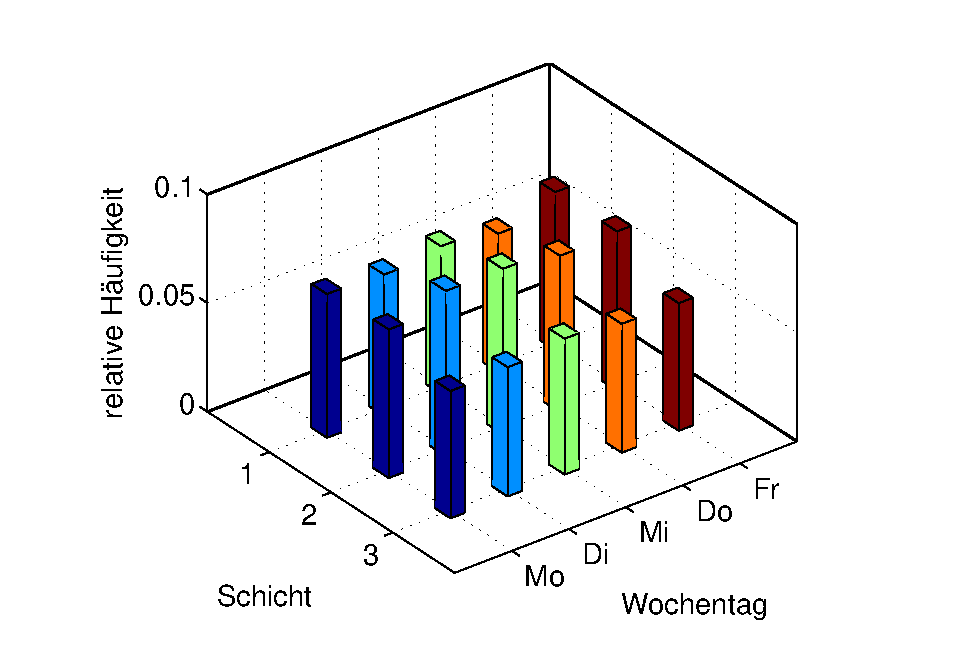
\includegraphics[width=0.5\textwidth]{Einleitung/Bilder/image1}}
  \caption{Systemtheorie Online (www.hs-karlsruhe.de/mesysto)}
  \label{fig:SYSONLINE}
\end{figure}
\bigskip

{\fontfamily{phv}\selectfont
\noindent\textbf{Applikationen zur Systemtheorie}} \smallskip

\noindent Für Sachverhalte und Zusammenhänge, die sich die Studierenden nur schwer vorstellen können, werden Applikationen zur Verfügung gestellt. Bei den Applikationen können Parameter beispielsweise per Schiebregler verändert und die Folgen dieser Modifikationen auf die Ausgabesignale beobachtet werden. Die Applikationen erlauben es, im Rahmen des spielerischen Ausprobierens ein Gefühl für Zusammenhänge und Abhängigkeiten verschiedener Systemparameter zu bekommen. In Video-Tutorials werden die Studierende in den Umgang mit den Applikationen eingeführt. Sie sollen dabei vor der Manipulation von Parametern Hypothesen über zu erwartende Effekte auf das Gesamtsystem abgeben, bevor das Ergebnis-Feedback bezüglich des Zutreffens des eigenen Vorhersagen erfolgt.

\clearpage
\noindent Das Vorgehen bei den grafischen Animationen kann kurz an einem Beispiel erläutert werden: Ein sogenanntes PT2-Glied ist von den Parametern Zeitkonstante T, Dämpfung d und Verstärkung k abhängig (Bild \ref{fig:PT2GLIED}). Die grafische Animation zeigt parallel die Eigenschaften des Systems im Zeit-, Laplace- und Frequenzbereich. Die Parameter können dabei durch Schieberegler variiert werden, sodass die Studierenden spielend ein Fingerspitzengefühl für das Übertragungsverhalten bekommen. Durch die Bereitstellung als Silverlight-Applikation benötigen die Studierenden keine zusätzliche Software, um das Programm auszuführen.

\begin{figure}[H]
  \centerline{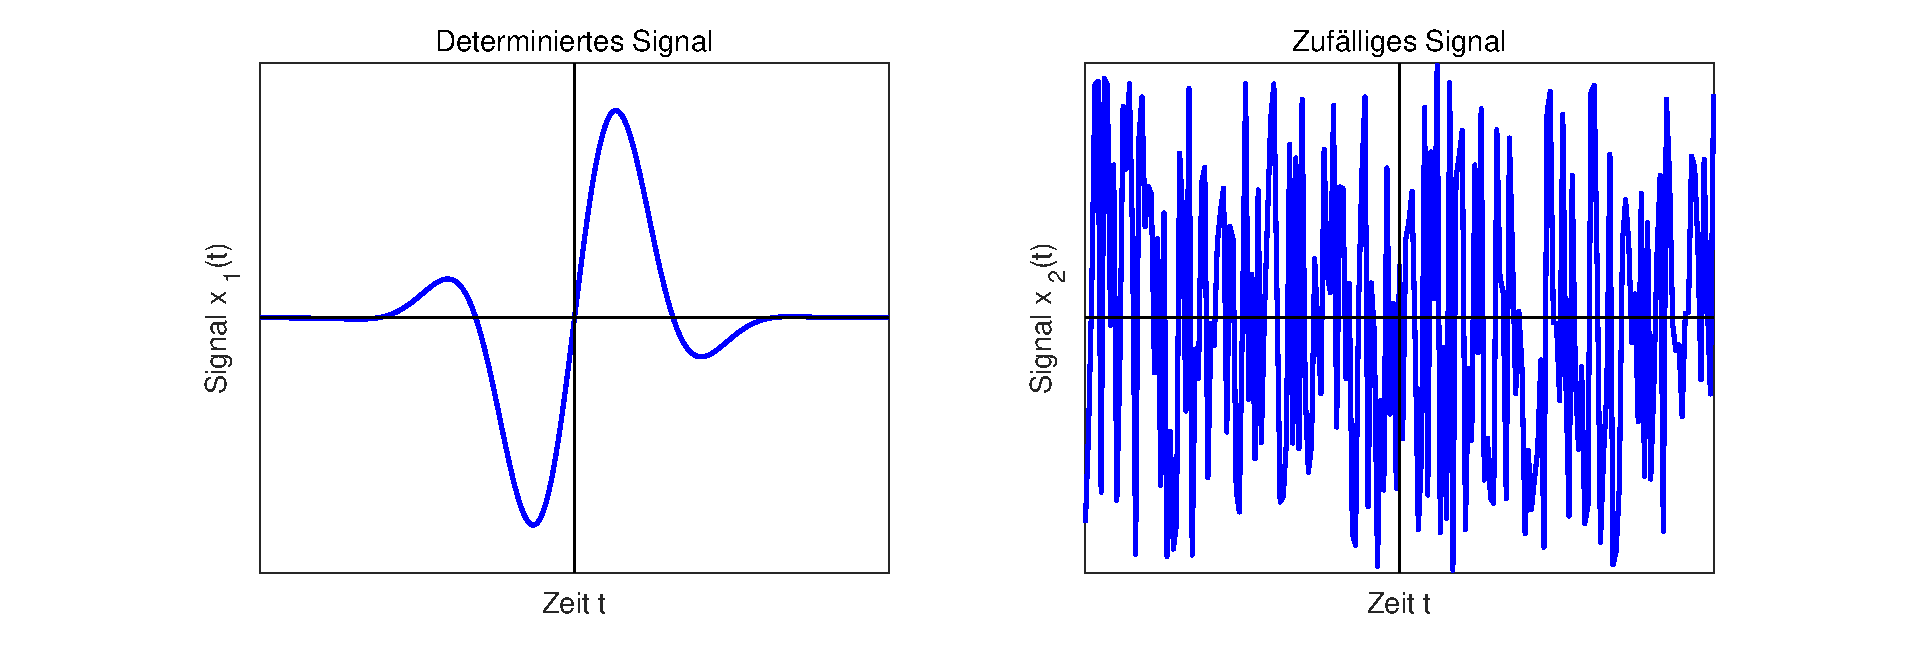
\includegraphics[width=0.5\textwidth]{Einleitung/Bilder/image2}}
  \caption{Darstellung des Verhaltens eines sogenannten PT2-Gliedes als Silverlight-Applikation}
  \label{fig:PT2GLIED}
\end{figure}

\noindent Da Microsoft die Wartung von Silverlight eingestellt hat, werden die verfügbaren Applikationen derzeit neu implementiert. Bild \ref{fig:Fourier-Reihe} zeigt eine erste Applikation, die unabhängig vom Betriebssystem lauffähig ist.

\begin{figure}[H]
  \centerline{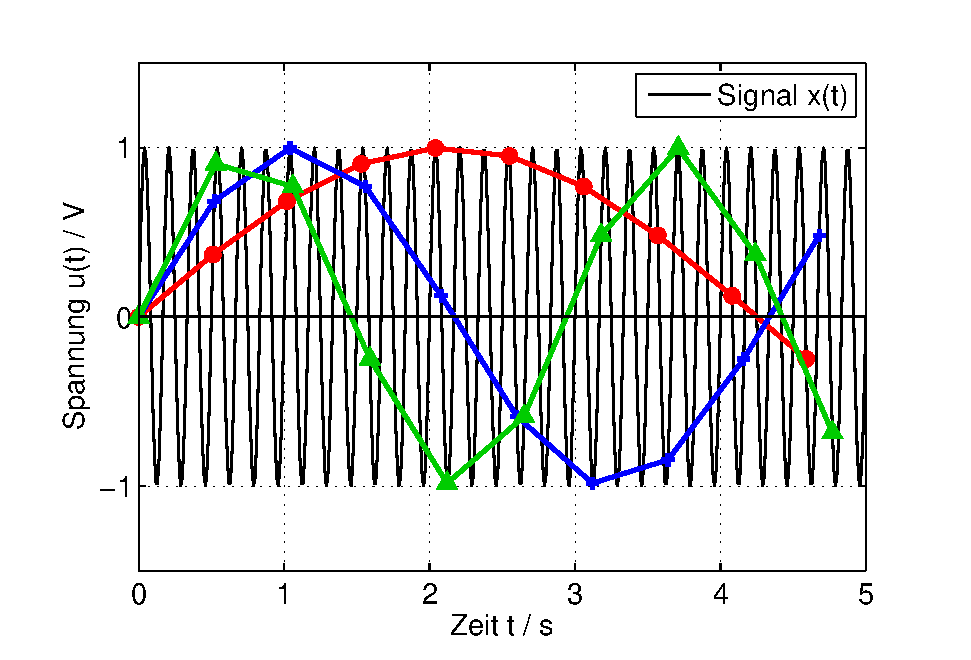
\includegraphics[width=0.5\textwidth]{Einleitung/Bilder/image3}}
  \caption{Applikation Fourier-Reihe}
  \label{fig:Fourier-Reihe}
\end{figure}

\noindent Bis zur kompletten Umsetzung können die Silverlight Applikationen mit dem Microsoft Internet Explorer weiterverwendet werden.\bigskip

{\fontfamily{phv}\selectfont
\noindent\textbf{Virtuelle Versuche zur Systemtheorie}} \smallskip

\noindent Darüber hinaus ermöglicht die Online-Plattform die Durchführung virtueller Experimente. Passend zu den Themen des Skripts werden Versuche mit dem Laborwagen auf Video aufgezeichnet und diese auf der Online-Plattform gemeinsam mit den entsprechenden Datensätzen zur Verfügung gestellt. Zusätzliche Erläuterungen zur Durchführung der Versuche und Auswertung der Daten fördern ein Grundverständnis für das wissenschaftliche Denken und Arbeiten. \newline
Als Experimente zur Demonstration stehen bereits einige Versuche mit dem Laborwagen zur Verfügung. Bild \ref{fig:EinschwingverhaltenLautsprecher} zeigt zum Beispiel einen Versuch zur Beschreibung des Einschwingverhaltens eines Lautsprechers. Weitere Experimente insbesondere zu den Themen zeitdiskrete Systeme und stochastische Systeme wurden aufgebaut und gefilmt, die Videos stehen als Datei zur Verfügung. Die Studierenden erhalten aber nicht nur den Video-Stream, sondern auch die einzelnen Versuchsergebnisse in Form von Daten-Files und können bei Interesse eigene Versuchsauswertungen erstellen

\begin{figure}[H]
  \centerline{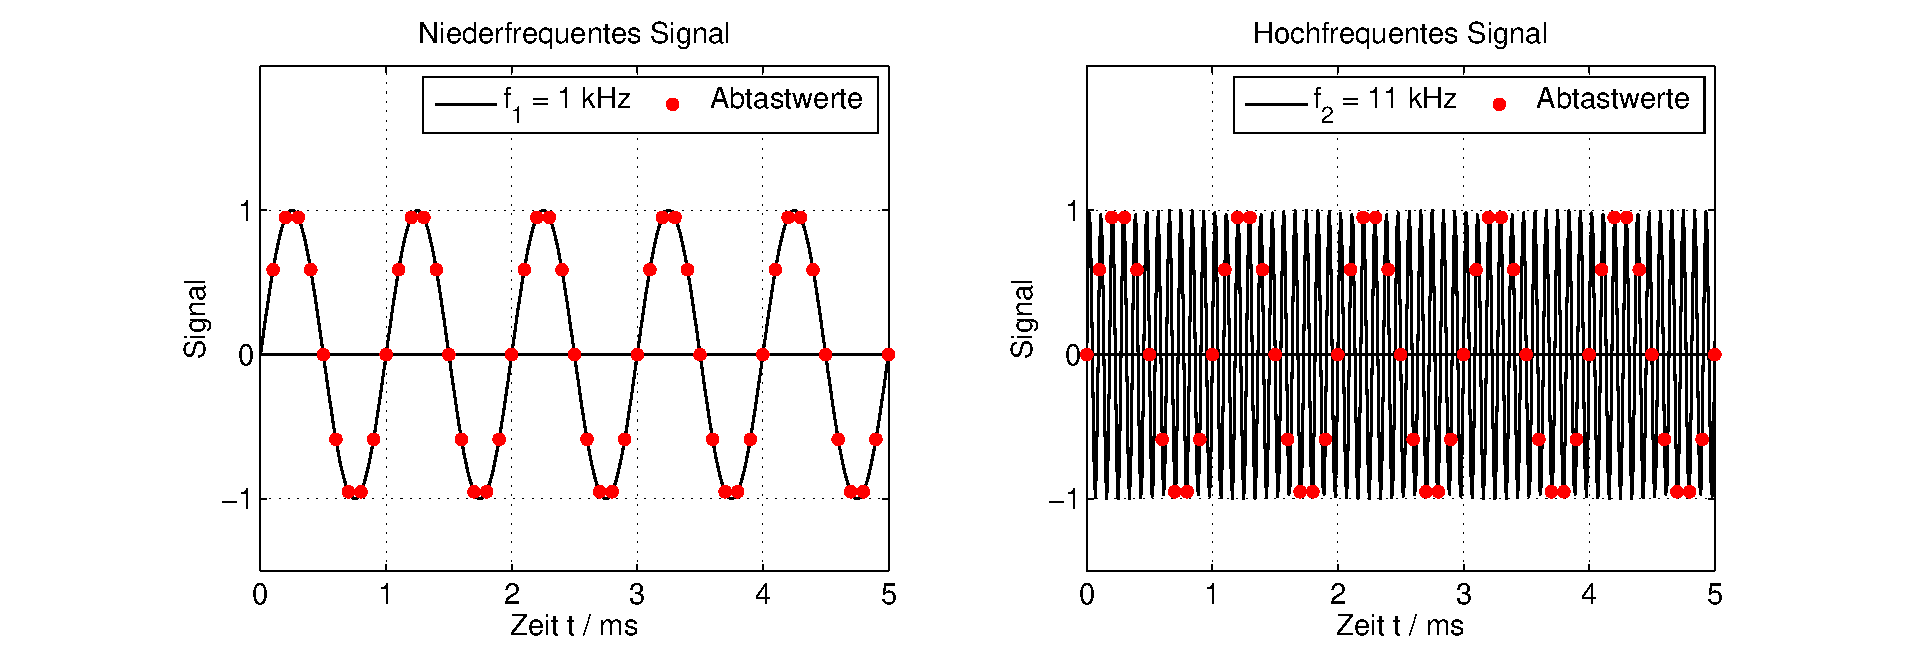
\includegraphics[width=0.5\textwidth]{Einleitung/Bilder/image4}}
  \caption{Versuchsaufbau zum Einschwingverhalten eines Lautsprechers}
  \label{fig:EinschwingverhaltenLautsprecher}
\end{figure}

\noindent Das Portal Systemtheorie-Online bietet den Studierenden damit die Möglichkeit, theoretische Sachverhalte auf eine anschauliche Art aufbereitet und erklärt zu bekommen. Damit wird eine Forderung aus der Evaluation aufgegriffen, mehr Versuche in der Systemtheorie einzusetzen. Darüber hinaus haben die Studierenden die Möglichkeit, selbst aktiv zu werden und Versuche selbstständig auszuwerten und daran ihren eigenen Lernerfolg zu messen. Das Projekt bietet da-mit einen Beitrag zur praxisnahen Ausbildung von Studierenden und stellt wegen des freien Zu-gangs ein Weiterbildungsangebot dar, das Mitarbeitern aus Industrie und Wirtschaft offensteht. Der Aufbau dieses Portals wurde im Rahmen von Pro-Studium aus Studiengebühren und aus Mitteln des Landes Baden-Württemberg im Rahmen des Programms Willkommen in der Wissenschaft finanziert.

\subsubsection{Teamorientierte Lehrmethoden}

\noindent Parallel zu den Online-Aktivitäten wird die Vorlesung um unterschiedliche teamorientierte Lehrmethoden ergänzt. Kooperative Lernformen fördern den Zusammenhalt und tragen sozialen Bedürfnissen Rechnung. Sie wirken der sozialen Isolation entgegen, die Studierenden fühlen sich eingebunden. Nicht zuletzt spiegelt die Teamarbeit auch berufliche Anforderungen wider. Die Methoden des teamorientierten Lernens sind auf der Online-Plattform ausführlich dokumentiert
\bigskip

{\fontfamily{phv}\selectfont
\noindent\textbf{Lange Nächte der Systemtheorie}} \smallskip

\noindent Lange Nächte sind abendliche Veranstaltungen zur Vertiefung des Vorlesungsstoffs, passend zu einem bestimmten Vorlesungsthema. In entspannter Atmosphäre werden Übungsaufgaben und Experimente mit dem Laborwagen miteinander kombiniert. Der verfügbare Zeitrahmen erlaubt eine Beschäftigung mit komplexeren Fragestellungen. In erster Linie ist dieser Baustein als offener Lernraum konzipiert, in dem Wissen stressfrei vermittelt und vertieft wird. Erste lange Nächte wurden von den Studierenden sehr positiv bewertet. Besonders gelobt wurden das gemeinschaftliche Lernen in der Gruppe, das angenehme Arbeitsklima sowie der Praxisbezug und die Arbeit mit realen Messdaten\bigskip

{\fontfamily{phv}\selectfont
\noindent\textbf{Großer Preis der Systemtheorie}} \smallskip

\noindent In Anlehnung an die Fernsehsendung "Der große Preis" wird mit den Studierenden eine Quiz-Show veranstaltet. Dabei bearbeiten die Studierenden in Gruppen Fragen zu Themenblöcken der Vorlesung. Die Punktzahl ist abhängig von Schwierigkeitsgrad. Die Abschätzung eines Einsatzes bei sogenannten RisikoFragen erfordert die Selbsteinschätzung der Studierenden. Durch sogenannte Glücksfragen zu fachfremden Themen können auch Gruppen mit mäßigem Fachwissen gewinnen. Die traditionelle Rangordnung innerhalb der Vorlesung wird aufgebrochen und die Motivation der Studierenden steigt. Studierenden zeigten bei der ersten Durchführung eine extrem hohe Motivation und hohes Engagement.\bigskip

{\fontfamily{phv}\selectfont
\noindent\textbf{Zirkeltraining Systemtheorie}} \smallskip

\noindent Erfolgreiches Lernen setzt ein Gleichgewicht zwischen Anspannung und Entspannung voraus. Zielsetzung dieses Zirkeltrainings ist es deshalb, sportliche Übungen oder Geschicklichkeitsspiele in den Lernprozess zu integrieren. Dazu wird ein Parkour aufgebaut, bei dem sich Übungsaufgaben und Spielstationen abwechseln. Bei der Veranstaltung stehen die Motivation und der Spaß an vorderster Stelle. Es wird eine angenehme Atmosphäre geschaffen, in der der Druck beim Bewältigen von Übungsaufgaben durch spielerische Anteile entlastet wird. Wegen des erforderlichen Platzbedarfs eignet sich das Zirkeltraining Systemtheorie insbesondere für die Sommermonate.\newline

\noindent Die Evaluationsergebnisse zur Vorlesung zeigen, dass es durch den Einsatz teamorientierter Lehrmethoden gelungen ist, diese Abneigung gegen das Fach Systemtheorie zumindest teilweise abzubauen

\clearpage

\subsection{Danksagung}

Wir bedanken uns bei den Studierenden und Assistenten Andreas Kühn, Erik Seiter, Sebastian Stiegler, Philipp Fetzer, Jaruwan Limsukhakorn, Doraemon Dedkum, Georg Bauer, Jochen Lang, Alex Schwin und Michael Holz für die Gestaltung und Ausarbeitung des wesentlichen Teils der Übungsaufgaben, Applikationen und Versuche.\newline
Unserer besonderer Dank gilt außerdem den Kollegen Prof. Dr. Beucher, Prof. Dr. Dussel, Prof. Dr. Quint und Prof. Dr. Weizenecker, die die inhaltliche und mathematische Darstellung in die-sem Buch kritisch hinterfragt und damit zur besseren Verständlichkeit beigetragen haben. \newline
In das Buch sind viele Hinweise von Studierenden der Hochschule Karlsruhe eingegangen. Wir haben versucht, den Hinweisen gerecht zu werden, die meisten Hinweise sind bereits in Überar-beitungen Korrekturen eingeflossen. Über weitere Hinweise zur mangelhaften Verständlichkeit und auf Fehler würden wir uns freuen. \newline

\noindent Karlsruhe, 15.03.2020

